\documentclass[journal=jcisd8,manuscript=article]{achemso}

\usepackage[T1]{fontenc}
\usepackage{graphicx}
\usepackage{booktabs}
\usepackage{amsmath}
\usepackage{amssymb}
\usepackage{array}
\usepackage{multirow}
\usepackage{url}

\SectionNumbersOn
\setkeys{acs}{articletitle=true}
\graphicspath{{figures/}}

\title{StructRSMA: A Proof-of-Concept Framework for PDB-Derived Contact-Supervised Transfer in RNA-Small Molecule Binding Affinity Prediction}

\author{First Author}
\affiliation{Department of Bioinformatics, Placeholder University, Placeholder City, Placeholder Country}
\author{Second Author}
\affiliation{Department of Pharmaceutical Sciences, Placeholder University, Placeholder City, Placeholder Country}
\author{Corresponding Author}
\affiliation{Department of Bioinformatics, Placeholder University, Placeholder City, Placeholder Country}
\email{corresponding.author@example.com}

\keywords{RNA-small molecule interaction, binding affinity prediction, structural supervision, contact map, multiview learning, graph neural network, interpretability}

\begin{document}

\begin{abstract}
RNA-small molecule affinity datasets usually provide only pair-level affinity labels, which makes it difficult for multiview models to learn local nucleotide-atom recognition patterns. To explore whether external structural information can alleviate this limitation, we present StructRSMA as a proof-of-concept contact-supervised transfer framework built on the DeepRSMA backbone. StructRSMA preserves the original four-branch RNA sequence, RNA graph, molecule sequence, and molecule graph encoders, and introduces PDB-derived nucleotide-atom contact supervision as an auxiliary structural learning signal. In the first stage, RNA-ligand complexes from PDB are converted into binary contact maps using a 4 \AA{} distance cutoff, and a contact prediction head is trained to learn local RNA-ligand contact patterns. In the second stage, the contact-pretrained backbone is transferred to R-SIM affinity prediction, where no contact labels are available. The pretrained contact head is reused to infer contact probability maps, and a lightweight Structural Contact Adapter (SCA) summarizes the inferred contact prior to perform residual calibration of the base affinity prediction. Under a controlled local independent-test reproduction protocol, Contact500 pretraining improved the reproduced DeepRSMA baseline from PCC 0.4866 and RMSE 1.0584 to PCC 0.5816 and RMSE 0.9152. SCA further reduced RMSE to 0.8518 under the best-RMSE checkpoint-selection view while maintaining comparable correlation metrics. De-overlap and random-SCA controls indicate that the observed behavior depends on both structural supervision and the coverage of the PDB pretraining set. These results support PDB-derived contact supervision as a structural signal that can transfer under the present data distribution, while also revealing its distributional sensitivity.
\end{abstract}

\section{Introduction}

RNA participates in transcription, translation, splicing, gene regulation, and catalysis, and its folded structures create pockets and surfaces that can be recognized by drug-like small molecules.\cite{Caprara2000RNA,ChildsDisney2022TargetingRNA,Warner2018Principles} The therapeutic relevance of RNA has motivated active efforts to discover small molecules that modulate RNA function, including compounds targeting riboswitches, viral RNA elements, splicing regulators, and disease-associated RNA structures.\cite{Costales2020How,Yu2020RNADrugs} However, measuring RNA-ligand binding affinity experimentally remains costly and time-consuming, which makes computational prioritization valuable in early RNA-targeted drug discovery.\cite{Kairys2019BindingAffinity}

Early computational studies for RNA-ligand recognition used docking and physics-inspired scoring functions to estimate binding poses or interaction energies.\cite{Guilbert2008DockingRNA,Feng2020ITScoreNL} Recent machine learning approaches have used molecular fingerprints, structural interaction fingerprints, target-specific models, and RNA subtype-aware predictors to model RNA-small molecule interactions.\cite{Grimberg2022MLRNA,Szulc2023FingeRNAt,Krishnan2024RSAPred} The R-SIM database further enabled data-driven RSMA modeling by collecting quantitative binding affinities for RNA-small molecule pairs.\cite{Krishnan2023RSIM} Building on this resource, DeepRSMA introduced a cross-fusion deep learning architecture with RNA sequence, RNA graph, small-molecule sequence, and small-molecule graph views, demonstrating that fine-grained sequence and graph information can improve affinity prediction.\cite{Huang2024DeepRSMA} DeepMIF and other multiview models further emphasized the importance of view-level interaction modeling for RSMA prediction.\cite{Song2026DeepMIF,Wu2025MultiviewRNA}

Despite these advances, a central limitation remains: most affinity datasets supervise models only with a global p$K_d$ label for each RNA-ligand pair. Such weak supervision requires the model to infer local physical recognition patterns indirectly from pair-level regression signals. This is difficult for two reasons. First, the available affinity data are small compared with protein-ligand resources. Second, binding affinity depends on sparse nucleotide-atom interactions, whereas the loss function treats the whole RNA-ligand pair as one scalar target. As a result, a model may predict p$K_d$ reasonably well without learning where the ligand contacts the RNA, limiting interpretability and downstream use in structure-guided design.

PDB RNA-ligand complexes offer a complementary form of supervision. Although they are not always paired with quantitative affinity labels, they contain atomic coordinates from which nucleotide-atom contact maps can be derived automatically. These contact maps encode which RNA nucleotides are spatially close to which ligand atoms and therefore provide a direct training signal for local recognition. Binding-site prediction methods such as RLBind already show that RNA-ligand contact information is useful for enriching binding regions,\cite{Wang2023RLBind} but this structural signal has not been fully explored as a conditionally transferable prior for affinity prediction in the DeepRSMA framework.

Rather than replacing the DeepRSMA architecture or claiming a new benchmark-leading model, StructRSMA asks a complementary question: can experimentally solved RNA-ligand structures provide contact-level supervision that transfers under the current data distribution to affinity prediction datasets containing only pair-level labels? This framing separates the proposed contribution from purely architectural multiview fusion improvements. The goal is to preserve the original DeepRSMA backbone while introducing a structurally grounded auxiliary task and a lightweight residual calibration module.

Here, we propose StructRSMA, a PDB-derived contact-supervised transfer framework for RSMA prediction. StructRSMA keeps the DeepRSMA backbone intact, including its RNA sequence embedding branch, RNA graph embedding branch, molecular graph embedding branch, molecular sequence embedding branch, and cross-fusion module. We then add two components. First, a nucleotide-atom contact prediction head is trained on PDB-derived RNA-ligand contact maps, allowing the backbone to learn local physical contacts before affinity fine-tuning. Second, a Structural Contact Adapter (SCA) is attached after the contact-supervised backbone. SCA does not replace the base affinity predictor; instead, it summarizes inferred contact-prior statistics and learns a residual correction to the base affinity prediction. This design aims to preserve the established multiview backbone while testing, in a proof-of-concept manner, whether contact supervision can be transferred from structure-only PDB complexes to pair-level R-SIM affinity prediction.

The main contributions of this work are as follows. (i) We construct a PDB-derived nucleotide-atom contact dataset for RNA-ligand complexes using a simple 4 \AA{} distance rule and evaluate true-contact, shuffled-contact, and de-overlapped contact settings. (ii) We introduce a two-stage contact-supervised transfer strategy in which Contact500 pretrains the shared backbone and contact head, whereas R-SIM fine-tunes affinity prediction without contact labels. (iii) We propose SCA, a lightweight contact-prior-guided residual calibration module that adjusts the base DeepRSMA prediction without replacing the original backbone. (iv) We add leakage-aware and distributional sensitivity analyses, including de-overlapped contact pretraining and a random-SCA capacity control without PDB contact pretraining. (v) We provide a qualitative evidence chain with contact-map and 3D structure visualizations, connecting predicted high-probability contacts to RNA-ligand geometry.

\section{Materials and Methods}

\subsection{Task Definition}

Given an RNA sequence $R$ and a small molecule $M$, the goal is to predict the binding affinity $y$, represented as p$K_d$. For structural contact supervision, an RNA-ligand complex is converted into a binary contact map
\begin{equation}
C \in \{0,1\}^{p \times q},
\end{equation}
where $p$ is the number of RNA nucleotides and $q$ is the number of ligand heavy atoms. A nucleotide-atom pair is labeled positive if the minimum distance between any heavy atom in nucleotide $i$ and ligand heavy atom $j$ is below 4 \AA:
\begin{equation}
C_{ij} =
\begin{cases}
1, & d(i,j) < 4\ \text{\AA},\\
0, & \text{otherwise}.
\end{cases}
\end{equation}
The contact task is therefore a sparse binary matrix prediction problem, whereas the affinity task is a scalar regression problem.

\subsection{DeepRSMA Backbone Preserved in StructRSMA}

StructRSMA reuses the complete DeepRSMA multiview backbone rather than treating it as a black-box feature extractor. In this work, ``preserved backbone'' means that the original RNA feature extraction module, small-molecule feature extraction module, cross-fusion module, and base affinity prediction path are retained.\cite{Huang2024DeepRSMA} StructRSMA does not remove any of the four original views; instead, it adds contact supervision and SCA on top of the representations produced by this backbone.

\paragraph{RNA feature extraction module.}
The original DeepRSMA RNA module represents an RNA from two complementary views: a nucleotide sequence view and an intramolecular graph view. In the graph view, an RNA contact or secondary-structure-derived map is converted into a nucleotide graph. Each nucleotide is treated as a node, and edges encode predicted or derived RNA intramolecular contacts. The initial node features are nucleotide embeddings, and a graph attention network (GAT) updates each nucleotide by attention-weighted aggregation over its neighboring nucleotides.\cite{Velickovic2017GAT} This produces nucleotide-level graph representations
\begin{equation}
H_{RG} \in \mathbb{R}^{p \times d},
\end{equation}
where $p$ is the number of RNA nucleotides and $d$ is the hidden dimension. This branch is intended to capture structural neighborhood information that is not explicit in the linear RNA sequence.

In the sequence view, DeepRSMA combines trainable nucleotide embeddings with pretrained RNA-FM representations.\cite{Chen2022RNAFM} The nucleotide-level embeddings are then processed by one-dimensional convolutional blocks with multiple kernel sizes, allowing the model to capture local and multiscale sequence patterns. The resulting RNA sequence stream is
\begin{equation}
H_{RS} \in \mathbb{R}^{p \times d},
\end{equation}
which preserves a token-level representation for each nucleotide. Thus, before cross-fusion, the RNA side contains both $H_{RS}$ from sequence context and $H_{RG}$ from graph-structured context. Secondary-structure and RNA contact features can be generated from tools and resources such as ViennaRNA and bpRNA, while the original DeepRSMA implementation uses predicted RNA contact information as part of the RNA graph construction.\cite{Lorenz2011ViennaRNA,Danaee2018bpRNA,Huang2024DeepRSMA}

\paragraph{Small-molecule feature extraction module.}
The original DeepRSMA small-molecule module also keeps two views. In the graph view, the ligand SMILES string is converted into a molecular graph, where atoms are nodes and covalent bonds are edges. Atomic descriptors are used as node features, and graph convolutional networks (GCNs) propagate information over the molecular topology,\cite{Kipf2017GCN} generating atom-level graph representations
\begin{equation}
H_{MG} \in \mathbb{R}^{q \times d},
\end{equation}
where $q$ is the number of ligand atoms. In the sequence view, the SMILES string is tokenized and encoded by a Transformer-style sequence encoder with multihead self-attention and feed-forward layers.\cite{Vaswani2017Attention} This branch learns contextual representations of SMILES tokens:
\begin{equation}
H_{MS} \in \mathbb{R}^{s \times d},
\end{equation}
where $s$ is the SMILES token length. The two ligand views therefore provide atom-level topology through $H_{MG}$ and SMILES-level sequence semantics through $H_{MS}$.

\paragraph{Cross-fusion module.}
DeepRSMA then integrates the RNA and ligand views using a transformer-based cross-fusion module. Before cross-attention, graph-view and sequence-view segment embeddings are added to the corresponding streams so that the transformer can distinguish graph-derived tokens from sequence-derived tokens. The RNA-side input is composed of the RNA graph and sequence streams, and the molecule-side input is composed of the molecule graph and SMILES sequence streams. The cross-fusion transformer contains two parallel cross-attention directions: RNA-to-molecule attention uses RNA tokens as queries and ligand tokens as keys/values, whereas molecule-to-RNA attention uses ligand tokens as queries and RNA tokens as keys/values. Therefore, the attention matrix can model graph--graph, sequence--sequence, and cross-view pairs between RNA nucleotides and ligand tokens/atoms, rather than only within-entity self-attention.

For clarity, we denote the split cross-fused outputs as
\begin{equation}
\tilde{H}_{RS},\tilde{H}_{RG},\tilde{H}_{MS},\tilde{H}_{MG} =
\mathrm{CrossFusion}(H_{RS},H_{RG},H_{MS},H_{MG}).
\end{equation}
Here, each $\tilde{H}$ stream has already been updated with information from the opposite biomolecular entity through cross-attention.

\paragraph{Base affinity prediction path.}
StructRSMA also preserves the original DeepRSMA affinity aggregation path. In this path, cross-fused token streams are masked and mean-pooled to obtain four view-level vectors:
\begin{equation}
h_{RS}=\mathrm{Pool}(\tilde{H}_{RS}),\quad
h_{RG}=\mathrm{Pool}(\tilde{H}_{RG}),\quad
h_{MS}=\mathrm{Pool}(\tilde{H}_{MS}),\quad
h_{MG}=\mathrm{Pool}(\tilde{H}_{MG}).
\end{equation}
These vectors form the multiview representation $H=[h_{RS},h_{RG},h_{MS},h_{MG}]$ used by SCA. For the preserved base DeepRSMA predictor, RNA-side and molecule-side information is further summarized into pair-level vectors $h_R$ and $h_M$ by combining the original branch-level embeddings with their corresponding cross-fused embeddings. The two pair-level vectors are then concatenated and passed to the affinity MLP:
\begin{equation}
\hat{y}_{base} = \mathrm{MLP}_{aff}([h_R,h_M]).
\end{equation}
This base path is kept as the primary affinity predictor, and SCA later learns only a residual calibration on top of it.

\paragraph{Token-level branch added for contact prediction.}
On top of the preserved DeepRSMA backbone, StructRSMA adds a token-level contact branch. This branch retains the cross-fused states before pooling. Therefore, the nucleotide and atom embeddings are not additional external features; they are token-level outputs of the same cross-fusion backbone. Because the RNA sequence-view and graph-view streams are aligned by nucleotide position, the nucleotide token fusion module defines the embedding of nucleotide $i$ as
\begin{equation}
r_i = \frac{1}{2}(\tilde{H}_{RS,i}+\tilde{H}_{RG,i}).
\end{equation}
This produces the nucleotide sequence $r_1,r_2,\ldots,r_p$ for contact prediction. On the ligand side, contact labels are indexed by ligand atoms rather than SMILES tokens. Therefore, the atom-level token selection module takes the ligand atom representation from the cross-fused molecular graph stream:
\begin{equation}
m_j = \tilde{H}_{MG,j}.
\end{equation}
This produces atom embeddings $m_1,m_2,\ldots,m_q$. The SMILES sequence stream $\tilde{H}_{MS}$ is still used by the backbone, the cross-fusion module, and the pooled affinity/SCA branch, but it is not used as the atom-indexed contact token because SMILES tokens are not guaranteed to correspond one-to-one to ligand atoms. RNA and ligand graph streams are padded to fixed maximum lengths in implementation, and the corresponding masks are applied when computing the contact loss and contact-prior statistics.
We keep this backbone because the original DeepRSMA ablation showed that graph views, sequence views, and cross-fusion all contribute to the final prediction.\cite{Huang2024DeepRSMA}

\begin{figure}[t]
\centering
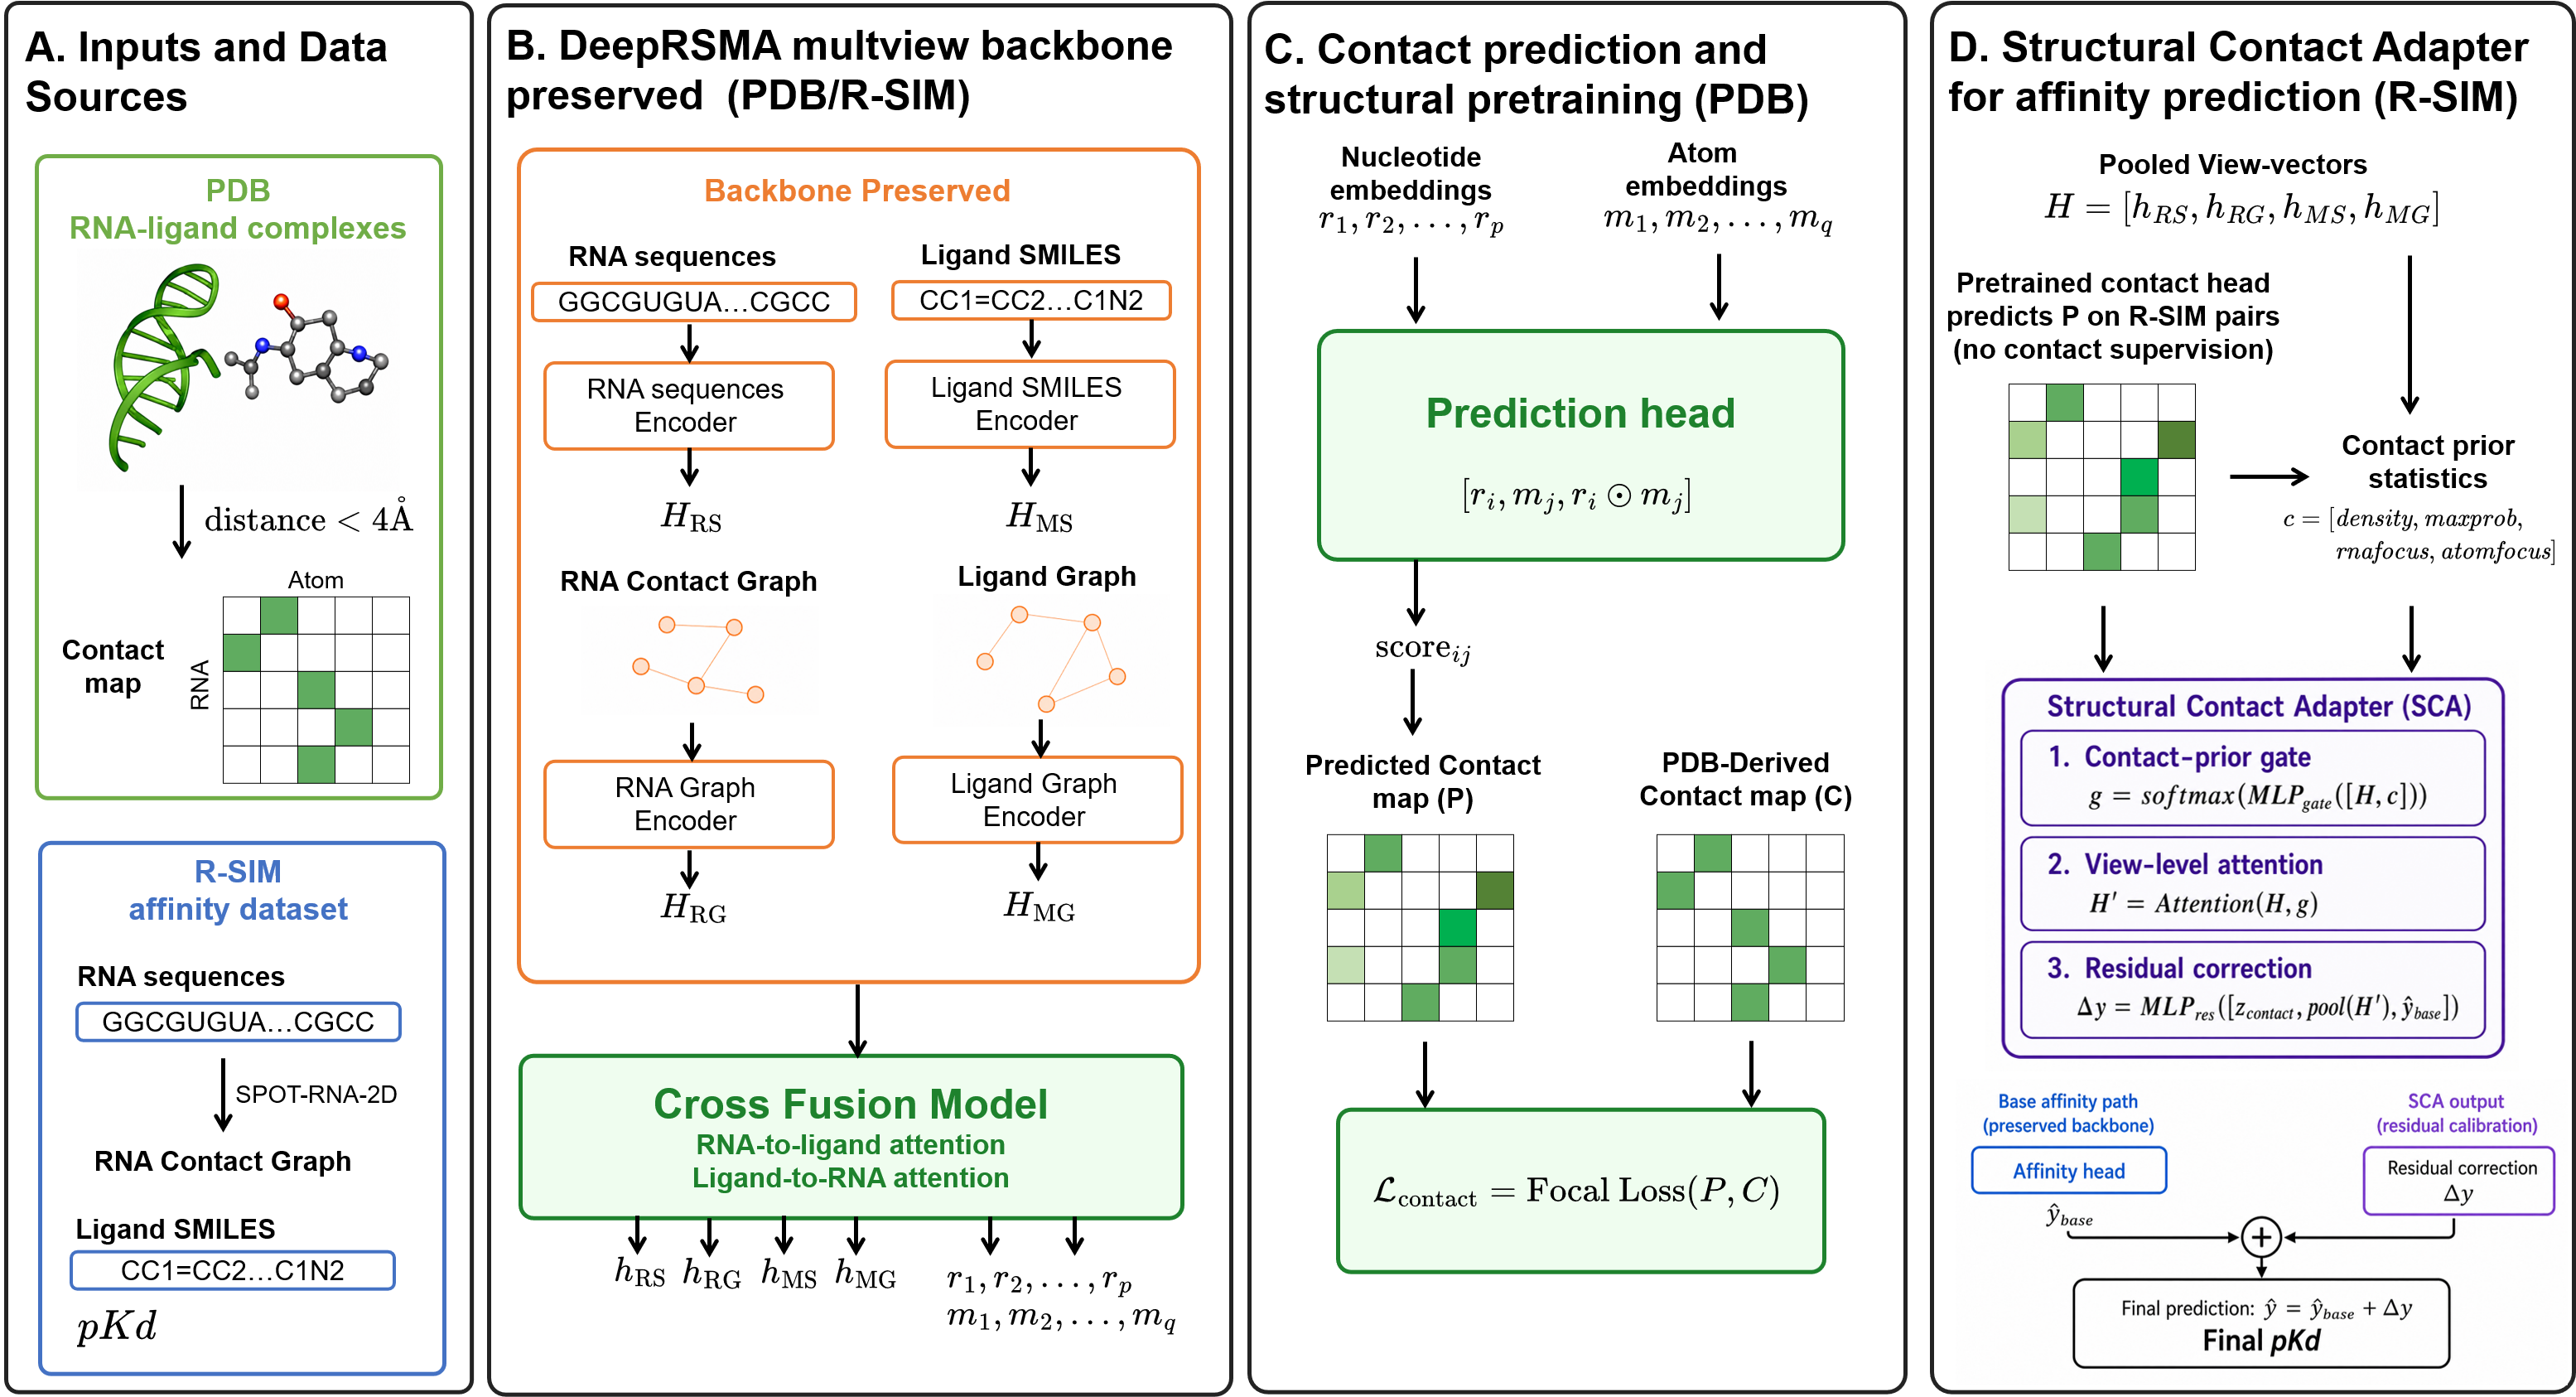
\includegraphics[width=0.95\linewidth]{overview.png}
\caption{Overview of StructRSMA. StructRSMA preserves the original DeepRSMA four-branch backbone and introduces PDB-derived nucleotide-atom contact supervision as an auxiliary structural pretraining task. In Stage 1, PDB RNA-ligand complexes are converted into contact maps and used to train the contact prediction head. In Stage 2, R-SIM provides only pair-level p$K_d$ labels; therefore, no contact labels are used. The pretrained contact head infers contact probability maps for R-SIM pairs, and SCA summarizes the inferred contact prior to predict a residual correction to the base affinity output.}
\label{fig:overview}
\end{figure}

\subsection{PDB-Derived Contact Dataset}

RNA-ligand complexes were extracted from PDB structures containing RNA polymer chains and nonpolymeric ligands. Water molecules, common ions, ambiguous ligands, and samples without valid RNA-ligand proximity were filtered. For each remaining complex, RNA nucleotide coordinates and ligand heavy-atom coordinates were parsed, and a nucleotide-atom contact map was generated using the 4 \AA{} rule described above. Each contact sample contains an RNA sequence, ligand identity or SMILES where available, ligand graph, and a binary contact map.

The resulting Contact500 set contains 484 usable RNA-ligand contact samples. To assess potential overlap with the downstream affinity test set, we also generated a de-overlapped Contact500 subset by removing contact samples with high ligand similarity or high local RNA sequence identity to independent-test examples. Specifically, a PDB contact sample was excluded if the maximum Morgan fingerprint Tanimoto similarity between its ligand and any independent-test ligand was at least 0.80, or if the best local RNA window identity to the independent-test RNA sequence was at least 0.80. This procedure removed 44 samples, including 36 samples with ligand Tanimoto similarity above the threshold, 23 exact ligand matches, and 8 samples with high local RNA identity. The de-overlapped subset contains 440 contact samples, with a maximum retained ligand Tanimoto similarity of 0.775 and a maximum retained local RNA identity of 0.793. This subset is used as a leakage-aware sensitivity control to examine how much contact-supervised transfer depends on structural coverage and proximity to the downstream test distribution.

Importantly, Contact500 and R-SIM serve different roles in StructRSMA. Contact500 is a newly introduced structural-supervision dataset; it is not an alternative affinity dataset and does not provide p$K_d$ labels. Its PDB coordinates are used only to derive nucleotide-atom contact maps. R-SIM, in contrast, provides pair-level binding affinity labels but does not provide nucleotide-atom contact annotations. After preprocessing, both data sources are represented as compatible RNA-ligand inputs and are passed through the same StructRSMA backbone, but they supervise different prediction heads. Thus, the transfer from PDB contact pretraining to R-SIM affinity prediction is a transfer of model parameters and structural inductive bias, not a direct transfer of PDB sample embeddings or contact labels.

\begin{table}[t]
\centering
\caption{Different roles of the PDB-derived contact data and R-SIM affinity data in StructRSMA.}
\label{tab:data_roles}
\small
\begin{tabular}{>{\raggedright\arraybackslash}p{0.17\linewidth}>{\raggedright\arraybackslash}p{0.25\linewidth}>{\raggedright\arraybackslash}p{0.23\linewidth}>{\raggedright\arraybackslash}p{0.25\linewidth}}
\toprule
Dataset & Source & Supervision label & Training role \\
\midrule
Contact500 & PDB RNA-ligand complexes & Nucleotide-atom contact map $C$ & Pretrain the shared backbone and contact head \\
R-SIM & Measured RNA-small molecule affinities & Pair-level p$K_d$ value $y$ & Fine-tune the affinity head/SCA for p$K_d$ prediction \\
\bottomrule
\end{tabular}
\end{table}

\begin{figure}[t]
\centering
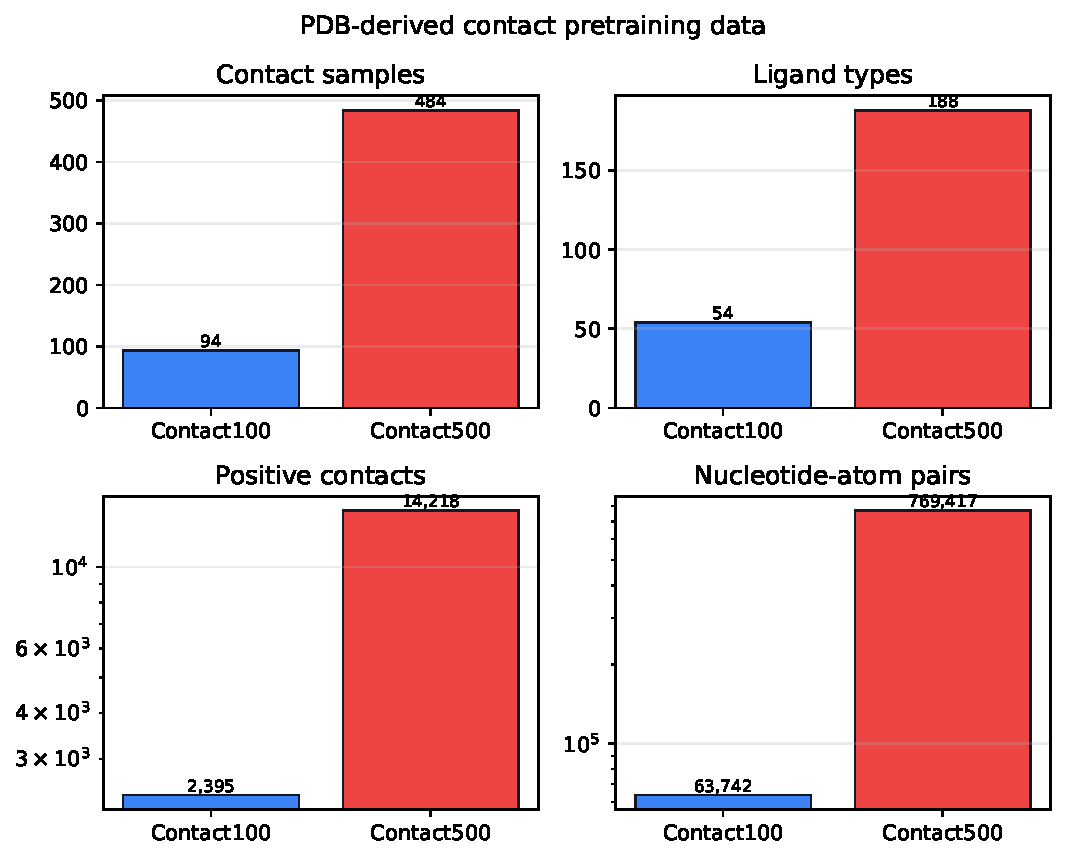
\includegraphics[width=0.88\linewidth]{fig_contact_dataset_summary.pdf}
\caption{Statistics of the PDB-derived contact dataset. Contact supervision converts RNA-ligand structures into nucleotide-atom matrices, providing local interaction labels that are absent from pair-level affinity datasets such as R-SIM.}
\label{fig:contact_dataset}
\end{figure}

\subsection{Contact Prediction Head and Loss}

Using the token definitions above, the contact head predicts a pairwise score between cross-fused nucleotide embedding $r_i$ and ligand atom embedding $m_j$:
\begin{equation}
s_{ij} = \mathrm{MLP}_{contact}([r_i,m_j,r_i \odot m_j]),
\end{equation}
where $\odot$ denotes elementwise multiplication. Scores over all nucleotide-atom pairs form a contact logit matrix $S \in \mathbb{R}^{p \times q}$. The contact probability matrix is $P=\sigma(S)$.

Because only a small fraction of nucleotide-atom pairs are contacts, contact prediction is highly imbalanced. We therefore use focal loss:
\begin{equation}
\mathcal{L}_{contact}
= -\alpha(1-p_t)^\gamma \log(p_t),
\end{equation}
with $\alpha=0.75$ and $\gamma=2.0$. This loss emphasizes difficult positive examples and reduces the dominance of the numerous negative pairs.

\subsection{Two-Stage Contact-Supervised Transfer}

StructRSMA is trained as a contact-supervised transfer framework. In Stage 1, Contact500 is used only for structural contact pretraining. Each PDB RNA-ligand complex provides a binary nucleotide-atom contact map, but no affinity label is used. The shared encoders, cross-fusion module, and contact prediction head are optimized with focal loss:
\begin{equation}
R,M \rightarrow C, \qquad \mathcal{L}_{stage1} = \mathcal{L}_{contact}.
\end{equation}
This stage is intended to teach the backbone local RNA-ligand recognition patterns rather than global affinity calibration.

In Stage 2, the contact-pretrained parameters are transferred to R-SIM affinity prediction. R-SIM provides pair-level p$K_d$ labels but no nucleotide-atom contact annotations. Therefore, the contact head is not supervised by contact labels during this stage. In the base affinity fine-tuning setting, the contact-pretrained encoders and cross-fusion layers initialize the DeepRSMA backbone, while the affinity head is trained on R-SIM; the contact head is loaded but is not part of the base affinity forward path. In the SCA setting, the contact-pretrained contact head is kept fixed and is used only in inference mode to produce a contact probability matrix for each R-SIM RNA-ligand pair. This inferred map is summarized into contact-prior statistics for SCA. The affinity objective is
\begin{equation}
R,M \rightarrow \hat{y}, \qquad
\mathcal{L}_{affinity} = \mathrm{MSE}(\hat{y},y).
\end{equation}
At this point, each R-SIM RNA-ligand pair is encoded again by the same backbone using its own RNA and ligand inputs. The method does not reuse a stored embedding from a PDB complex. Instead, the RNA encoder, molecule encoder, and cross-fusion weights learned during contact pretraining initialize the R-SIM model, and the token-level representations are then pooled into pair-level vectors for affinity regression.
In the DeepRSMA + Contact500 pretraining setting, the contact-pretrained backbone is loaded while the affinity head is reinitialized or retrained on R-SIM. This avoids overinterpreting an affinity head that was not trained during contact-only pretraining and lets R-SIM determine the global p$K_d$ calibration. For the final StructRSMA-SCA experiments, the contact-pretrained backbone and the R-SIM affinity path are loaded from the corresponding checkpoints, all original parameters are frozen, and only the SCA residual adapter is optimized. The final layer of the residual branch is initialized to zero, so the SCA model starts from the base affinity prediction and learns an additive correction.

\subsection{Structural Contact Adapter}

After DeepRSMA + Contact500 pretraining and affinity fine-tuning, StructRSMA further introduces SCA. SCA is designed as a conservative residual calibration module rather than a replacement for the base DeepRSMA affinity predictor. Its purpose is not to build a new global representation from scratch, but to determine how the inferred contact prior should adjust the base prediction. It learns a residual correction conditioned on contact-prior statistics and the four pooled view vectors:
\begin{equation}
H=[h_{RS},h_{RG},h_{MS},h_{MG}].
\end{equation}
From the predicted contact probability matrix $P$, we compute four contact summary statistics:
\begin{equation}
c=[\mathrm{density},\mathrm{maxprob},\mathrm{rnafocus},\mathrm{atomfocus}].
\end{equation}
Let $V_{ij}$ denote the valid-pair mask after padding is removed. The four statistics are defined as
\begin{equation}
\mathrm{density}=\frac{\sum_{ij}P_{ij}V_{ij}}{\sum_{ij}V_{ij}}, \quad
\mathrm{maxprob}=\max_{V_{ij}=1}P_{ij},
\end{equation}
\begin{equation}
\mathrm{rnafocus}=\frac{\max_i\sum_jP_{ij}V_{ij}}{\sum_j V_{ij}}, \quad
\mathrm{atomfocus}=\frac{\max_j\sum_iP_{ij}V_{ij}}{\sum_i V_{ij}}.
\end{equation}
These statistics intentionally compress the full contact map into a small set of physically interpretable priors. Density approximates the overall predicted contact mass, reflecting the expected extent of the RNA-ligand interface. Maxprob captures whether a high-confidence local anchoring contact exists, which is often important for stable recognition. Rnafocus measures whether the predicted contact probability is concentrated on a small number of nucleotides, corresponding to a more localized RNA binding pocket. Atomfocus analogously measures whether the predicted interaction is concentrated on a few ligand atoms, which can reflect key pharmacophoric atoms or substituents. This compact representation sacrifices detailed pairwise geometry, but it reduces overfitting risk on the small R-SIM affinity set while still exposing the affinity model to contact strength, anchoring, and binding-pocket specificity.

SCA first computes a contact-prior-conditioned view gate:
\begin{equation}
g=\mathrm{softmax}(\mathrm{MLP}_{gate}([H,c])).
\end{equation}
The gated view representation is
\begin{equation}
z_{contact}=W_c\sum_{k=1}^{4} g_k h_k.
\end{equation}
In parallel, lightweight attention updates the four view vectors:
\begin{equation}
A=\mathrm{softmax}\left(\frac{Q(H)K(H)^T}{\sqrt{d}}\right), \qquad
H' = A V(H).
\end{equation}
The final SCA residual is predicted from the contact-guided vector, attended view summary, and base affinity prediction:
\begin{equation}
\Delta y = \mathrm{MLP}_{sca}([z_{contact},\mathrm{pool}(H'),\hat{y}_{base}]),
\end{equation}
\begin{equation}
\hat{y}_{StructRSMA} = \hat{y}_{base} + \Delta y.
\end{equation}
This design keeps the improvement tightly scoped: the original backbone remains available, while SCA learns how contact evidence should calibrate the final affinity estimate.

\subsection{Experimental Setup and Metrics}

Affinity prediction was evaluated using Pearson correlation coefficient (PCC), Spearman correlation coefficient (SCC), and root mean squared error (RMSE). PCC evaluates linear agreement between predicted and experimental p$K_d$, SCC evaluates rank-order agreement, and RMSE evaluates absolute regression error. Higher PCC and SCC are better, whereas lower RMSE is better.

Contact prediction was evaluated using top-$k$ precision, area under the precision-recall curve (AUPRC), and area under the receiver operating characteristic curve (AUROC). For each complex, $k$ was set to the number of ground-truth positive contacts, and top-$k$ precision measures the fraction of predicted top-$k$ pairs that are true contacts. This metric is suitable for sparse contact maps because it evaluates whether the model ranks true local interactions near the top. Because nucleotide-atom contact maps are highly sparse, top-$k$ precision and AUPRC are treated as the primary contact metrics, whereas AUROC is reported as a secondary metric that can be less sensitive under strong class imbalance.

We report means and standard deviations over three random seeds for the downstream affinity experiments. The reported affinity results are from a local independent-test reproduction protocol implemented from the available DeepRSMA-style training scripts. No official five-fold cross-validation experiment is claimed in this work. In the present submission, no internal validation-selected final model selection is used for the affinity experiments; instead, best-PCC, best-SCC, and best-RMSE are reported as retrospective checkpoint-selection views over the same independent-test trajectory. These views are used to diagnose whether a method mainly affects rank correlation or absolute error calibration. They should therefore be interpreted as proof-of-concept and sensitivity-analysis results, not as an unbiased estimate of fully held-out generalization. All compared local variants are summarized under the same rules. To examine possible cross-stage leakage and distributional dependence, we additionally fine-tuned affinity models initialized from the de-overlapped Contact500 checkpoint. To separate the effect of structure supervision from the effect of adding SCA parameters, we trained a random-SCA capacity control that loads a reproduced DeepRSMA affinity checkpoint, keeps the contact head randomly initialized, and trains only the SCA residual adapter with the same number of trainable adapter parameters.

\section{Results and Discussion}

\subsection{Contact Supervision Provides Learnable Local Structural Signal}

The first question is whether the PDB-derived contact maps contain a learnable signal. Because nucleotide-atom contact maps are highly sparse, we focus primarily on top-$k$ precision and AUPRC. AUROC is reported as a secondary metric because it can remain high under strong class imbalance. On Contact500 validation, the true-contact model achieved top-$k$ precision of 0.3471, AUPRC of 0.2847, and AUROC of 0.8828. The shuffled-label control had the same positive-contact density but broke the association between RNA-ligand geometry and labels, reducing top-$k$ precision to 0.0261 and AUPRC to 0.0571. This large gap indicates that the model is not merely exploiting label sparsity or matrix shape; it learns structured nucleotide-atom recognition patterns.

\begin{table}[t]
\centering
\caption{Contact prediction controls on PDB-derived RNA-ligand contact maps.}
\label{tab:contact_controls}
\begin{tabular}{lcccc}
\toprule
Setting & Samples & Top-$k$ precision & AUPRC & AUROC \\
\midrule
True Contact500 & 484 & 0.3471 & 0.2847 & 0.8828 \\
Shuffled Contact500 & 484 & 0.0261 & 0.0571 & 0.7327 \\
De-overlap Contact500 & 440 & 0.3817 & 0.3678 & 0.9408 \\
\bottomrule
\end{tabular}
\end{table}

\begin{figure}[t]
\centering
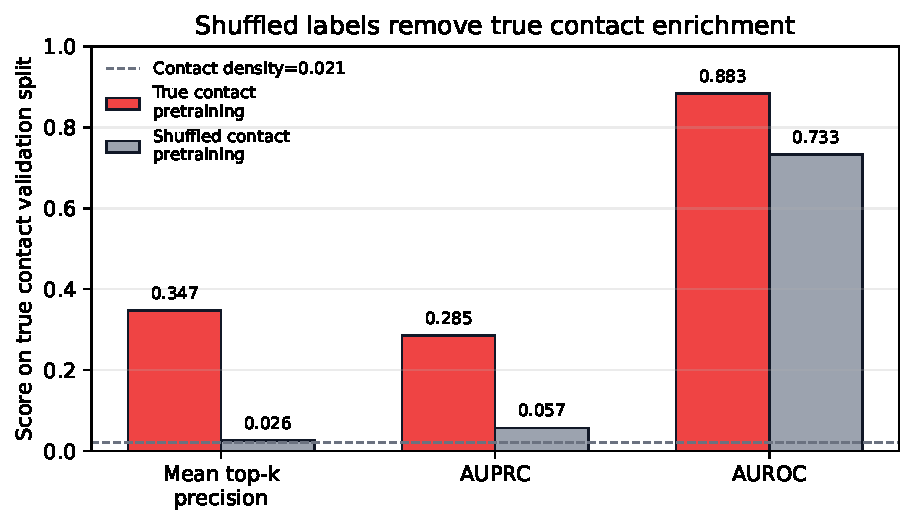
\includegraphics[width=0.88\linewidth]{fig_contact_shuffle_control.pdf}
\caption{True contact supervision versus shuffled-label control. Preserving the contact density while shuffling labels substantially reduces top-$k$ precision and AUPRC, supporting that the contact labels contain genuine structural information.}
\label{fig:contact_shuffle}
\end{figure}

The de-overlapped subset achieved top-$k$ precision of 0.3817, AUPRC of 0.3678, and AUROC of 0.9408. Although the de-overlap subset is smaller, the contact metrics remain strong, suggesting that the contact head captures nontrivial nucleotide-atom contact regularities even after removal of highly similar downstream-test neighbors.

\subsection{Contact Pretraining Improves Affinity Prediction under the Local Reproduction Protocol}

We next transferred the contact-pretrained backbone to R-SIM affinity prediction. In the local independent-test reproduction protocol, the reproduced DeepRSMA baseline achieved PCC 0.4866, SCC 0.4912, and RMSE 1.0584 under the best-PCC checkpoint-selection view. DeepRSMA + Contact100 pretraining improved PCC to 0.5195 and RMSE to 0.9754. Scaling contact pretraining to DeepRSMA + Contact500 pretraining further improved PCC to 0.5816 and RMSE to 0.9152. Within this local protocol, increasing the amount of PDB-derived contact supervision was associated with improved downstream affinity metrics.

\begin{table}[t]
\centering
\caption{Affinity prediction performance of contact-supervised variants in the local independent-test protocol. Values are mean $\pm$ standard deviation over three random seeds.}
\label{tab:affinity_contact}
\begin{tabular}{lccc}
\toprule
Method & PCC $\uparrow$ & SCC $\uparrow$ & RMSE $\downarrow$ \\
\midrule
Reproduced DeepRSMA & $0.4866 \pm 0.0522$ & $0.4912 \pm 0.0523$ & $1.0584 \pm 0.1490$ \\
+ Contact100 pretraining & $0.5195 \pm 0.0333$ & $0.5257 \pm 0.0194$ & $0.9754 \pm 0.0380$ \\
+ Contact500 pretraining & $0.5816 \pm 0.0547$ & $0.5749 \pm 0.0590$ & $0.9152 \pm 0.0788$ \\
\bottomrule
\end{tabular}
\end{table}

\begin{figure}[t]
\centering
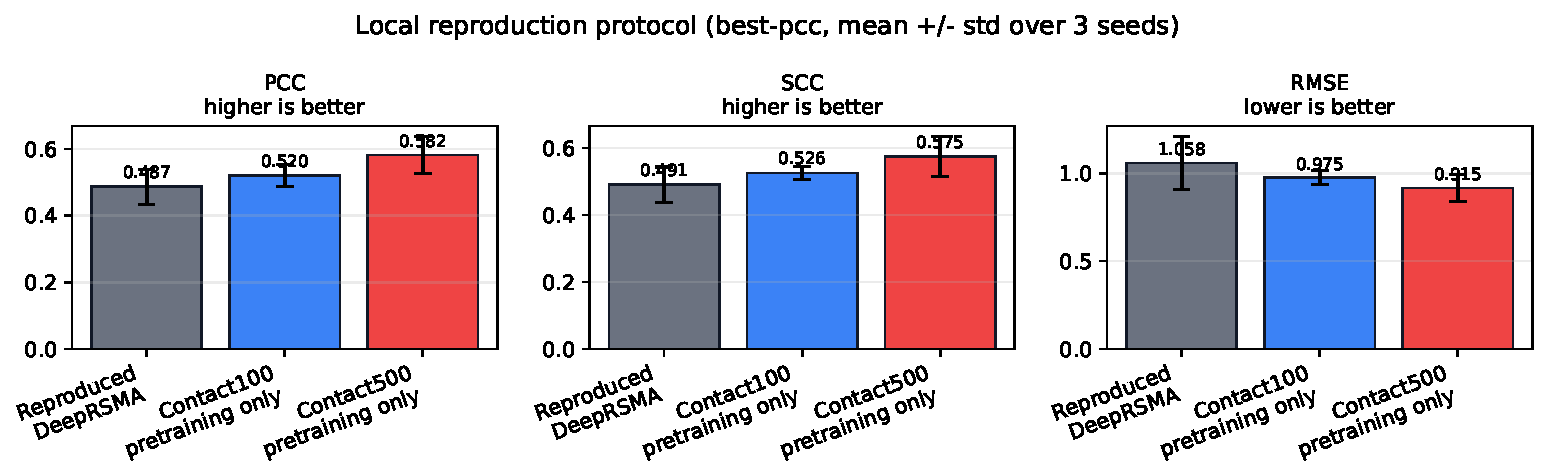
\includegraphics[width=0.88\linewidth]{fig_performance_best_pcc.pdf}
\caption{Downstream affinity performance under the best-PCC checkpoint-selection view. Under the local reproduction protocol, contact pretraining improves the reproduced DeepRSMA baseline, and the larger Contact500 set gives the strongest result among the tested contact-pretraining variants.}
\label{fig:best_pcc}
\end{figure}

When the checkpoint-selection view emphasizes RMSE, DeepRSMA + Contact500 pretraining also improves absolute error. The reproduced baseline achieved RMSE 0.9298, whereas Contact500 pretraining reduced RMSE to 0.8665. Shuffled-contact pretraining did not reproduce the same benefit and yielded worse RMSE than true-contact pretraining. This downstream control complements the contact-task control and suggests that the observed gain is associated with meaningful contact supervision rather than additional PDB pretraining steps alone.

\begin{figure}[t]
\centering
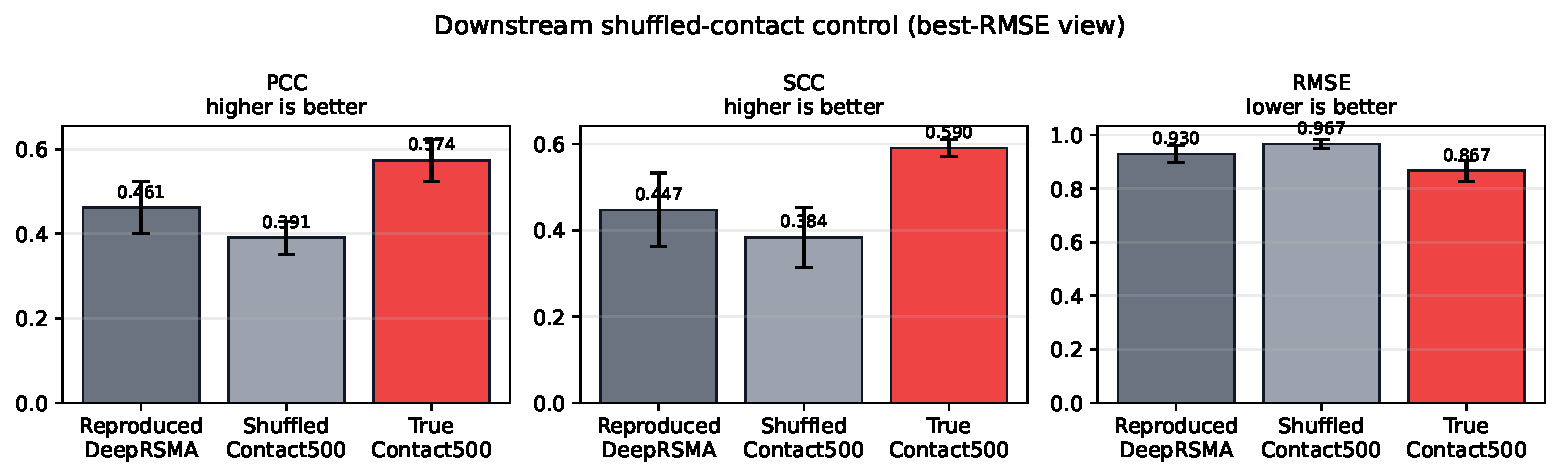
\includegraphics[width=0.88\linewidth]{fig_downstream_shuffle_control.pdf}
\caption{Downstream shuffled-control experiment. Under the local reproduction protocol, true Contact500 pretraining improves affinity prediction more consistently than shuffled-contact pretraining, suggesting that the geometric content of contact labels matters.}
\label{fig:downstream_shuffle}
\end{figure}

\subsection{De-overlapped Contact Pretraining Reveals Distributional Sensitivity}

Because PDB-derived contact pretraining and R-SIM affinity evaluation are performed in two stages, it is important to test whether the downstream gain depends on contact samples that are similar to independent-test examples. We therefore repeated the affinity transfer experiment using the de-overlapped Contact500 checkpoint described above. This control removes PDB contact samples whose ligands are highly similar to independent-test ligands or whose local RNA sequence windows are highly similar to the independent-test RNA sequence. We use this experiment as a leakage-aware and distributional sensitivity analysis rather than as proof that overlap has no effect.

\begin{table}[t]
\centering
\caption{Downstream affinity transfer with full Contact500 versus de-overlapped Contact500 pretraining. Values are mean $\pm$ standard deviation over three random seeds.}
\label{tab:deoverlap_affinity}
\small
\setlength{\tabcolsep}{3pt}
\begin{tabular}{lclccc}
\toprule
Pretraining set & Samples & Selection & PCC $\uparrow$ & SCC $\uparrow$ & RMSE $\downarrow$ \\
\midrule
Contact500 & 484 & best-PCC & $0.5816 \pm 0.0547$ & $0.5749 \pm 0.0590$ & $0.9152 \pm 0.0788$ \\
De-overlap Contact500 & 440 & best-PCC & $0.4161 \pm 0.0433$ & $0.3906 \pm 0.0604$ & $2.4148 \pm 2.1947$ \\
Contact500 & 484 & best-RMSE & $0.5738 \pm 0.0495$ & $0.5902 \pm 0.0204$ & $0.8665 \pm 0.0400$ \\
De-overlap Contact500 & 440 & best-RMSE & $0.3899 \pm 0.0282$ & $0.3389 \pm 0.0119$ & $0.9639 \pm 0.0132$ \\
\bottomrule
\end{tabular}
\end{table}

The de-overlapped contact checkpoint remained effective on the contact prediction task (Table~\ref{tab:contact_controls}), but it did not reproduce the full downstream affinity gain. Under best-RMSE selection, de-overlapped pretraining produced a stable RMSE of $0.9639 \pm 0.0132$, but its correlation metrics were lower than those of full Contact500 pretraining. Under best-PCC selection, one seed selected an early checkpoint with very large RMSE, yielding high variance. This negative control is important: it shows that the downstream benefit is not guaranteed by contact-task success alone, and that affinity transfer depends on the coverage and distributional proximity of the structural pretraining set. Therefore, the main Contact500 result should be interpreted as a local contact-supervised transfer result under the present data distribution, while the de-overlap experiment motivates larger and more diverse RNA-ligand structural datasets for leakage-robust transfer.

\subsection{SCA Provides Residual Calibration of Absolute Error}

Because SCA is designed as a residual calibration module, we report checkpoint-selection views based on PCC, SCC, and RMSE to distinguish ranking-oriented performance from absolute-error calibration. SCA was evaluated after the DeepRSMA + Contact500 pretraining model. Compared with the Contact500-pretrained best-PCC checkpoint, StructRSMA with SCA only slightly changed the correlation metrics but reduced RMSE from 0.9152 to 0.8696. Under best-SCC selection, StructRSMA reached SCC 0.6038 and RMSE 0.8671. Under best-RMSE selection, StructRSMA achieved RMSE 0.8518, the lowest error among the local variants tested. These results support SCA mainly as a residual calibrator of absolute p$K_d$ error rather than as a module that consistently increases ranking performance.

To determine whether this improvement comes merely from adding adapter parameters, we trained a random-SCA capacity control. This control loads a reproduced DeepRSMA affinity checkpoint, leaves the contact head randomly initialized, and trains the same SCA residual adapter without PDB contact pretraining. Random-SCA improved some seeds, indicating that adapter capacity and residual calibration can help. However, it was substantially less stable across seeds and remained below contact-pretrained StructRSMA-SCA on average, especially for RMSE calibration.

\begin{table}[t]
\centering
\caption{Effect of the Structural Contact Adapter and random-SCA capacity control. Values are mean $\pm$ standard deviation over three random seeds.}
\label{tab:sca_results}
\small
\setlength{\tabcolsep}{3pt}
\begin{tabular}{llccc}
\toprule
Method & Selection & PCC $\uparrow$ & SCC $\uparrow$ & RMSE $\downarrow$ \\
\midrule
+ Contact500 pretraining & init. best-PCC & $0.5816 \pm 0.0547$ & $0.5749 \pm 0.0590$ & $0.9152 \pm 0.0788$ \\
Random-SCA control & best-PCC & $0.5158 \pm 0.0986$ & $0.5014 \pm 0.0991$ & $0.9855 \pm 0.1390$ \\
Random-SCA control & best-SCC & $0.5116 \pm 0.0980$ & $0.5166 \pm 0.0860$ & $0.9611 \pm 0.0976$ \\
Random-SCA control & best-RMSE & $0.5134 \pm 0.0967$ & $0.5085 \pm 0.0818$ & $0.9294 \pm 0.0759$ \\
StructRSMA & best-PCC & $0.5870 \pm 0.0590$ & $0.5844 \pm 0.0663$ & $0.8696 \pm 0.0451$ \\
StructRSMA & best-SCC & $0.5786 \pm 0.0712$ & $0.6038 \pm 0.0428$ & $0.8671 \pm 0.0450$ \\
StructRSMA & best-RMSE & $0.5792 \pm 0.0602$ & $0.5873 \pm 0.0325$ & $0.8518 \pm 0.0419$ \\
\bottomrule
\end{tabular}
\end{table}

\begin{figure}[t]
\centering
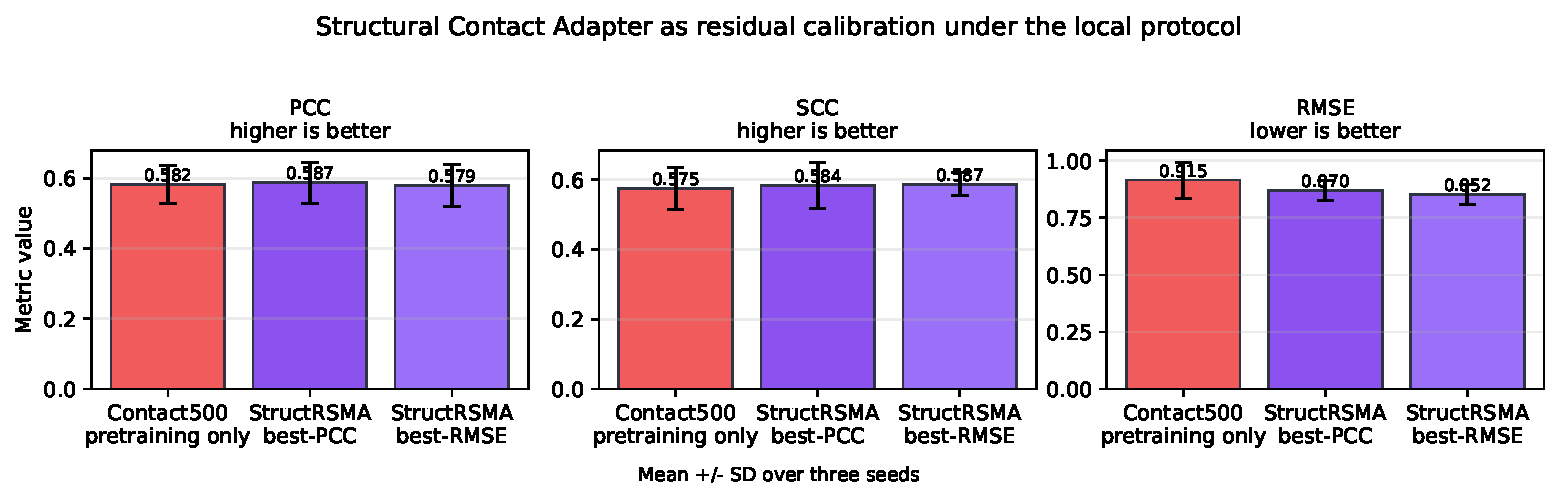
\includegraphics[width=0.9\linewidth]{fig_sca_adapter_results.pdf}
\caption{SCA results over three seeds. The adapter preserves the contact-supervised backbone and learns a residual calibration driven by contact-prior statistics and four-view molecular representations.}
\label{fig:sca_results}
\end{figure}

These results indicate that PDB-derived contact supervision affects the transferred DeepRSMA representation, while SCA primarily acts as a calibration module that reduces absolute prediction error. The random-SCA control further clarifies the mechanism: the adapter itself can contribute useful residual flexibility, but the contact-pretrained version provides a more stable and lower-error calibration signal. This is desirable for a conservative extension of DeepRSMA: the original backbone is kept, the contact-pretrained representation is retained, and the adapter learns a small correction informed by structural contact evidence. The improvement in RMSE is particularly relevant for virtual screening settings where the absolute p$K_d$ scale affects hit prioritization.

The current SCA intentionally uses compact contact-prior statistics rather than full pairwise contact-map attention. This design choice reflects the limited size of both Contact500 and R-SIM. A full contact-map-conditioned attention module would introduce substantially more parameters and could overfit under small-data conditions. In contrast, the proposed statistics provide a lightweight way to expose the affinity predictor to inferred structural evidence while keeping the original DeepRSMA representation stable.

\subsection{Qualitative Case Study: Contact Maps and 3D Structural Evidence}

To examine whether predicted contacts are enriched in physically relevant structural regions, we visualized a PDB case study for 3F4H with ligand RS3. The RNA has 54 nucleotides and the ligand has 29 heavy atoms. The ground-truth contact map contains 23 positive nucleotide-atom contacts involving 5 nucleotides and 16 ligand atoms. The model achieved top-$k$ precision of 0.435, corresponding to 10 true contacts among the top 23 predicted pairs.

\begin{figure}[t]
\centering

\includegraphics[width=0.95\linewidth]{fig_contact_map_example.pdf}
\caption{Contact-map case study for PDB 3F4H ligand RS3. The left panel shows ground-truth nucleotide-atom contacts, and the right panel shows predicted contact probabilities with top-$k$ true and false predictions annotated. The model partially recovers true-contact features by enriching probability mass near a subset of physically relevant nucleotide-atom pairs.}
\label{fig:contact_map_case}
\end{figure}

The contact matrix appears sparse and banded because only a few nucleotides are physically close to the ligand and because neighboring ligand atoms can share similar distances to the same nucleotide. This pattern is expected for nucleotide-atom contact maps: a single ligand-binding pocket often produces clusters of positive contacts across a small group of nucleotides and chemically adjacent ligand atoms. The predicted heatmap therefore should not be interpreted like an image segmentation mask; instead, high-probability rows and columns indicate candidate interacting nucleotides and ligand atoms.

\begin{figure}[t]
\centering
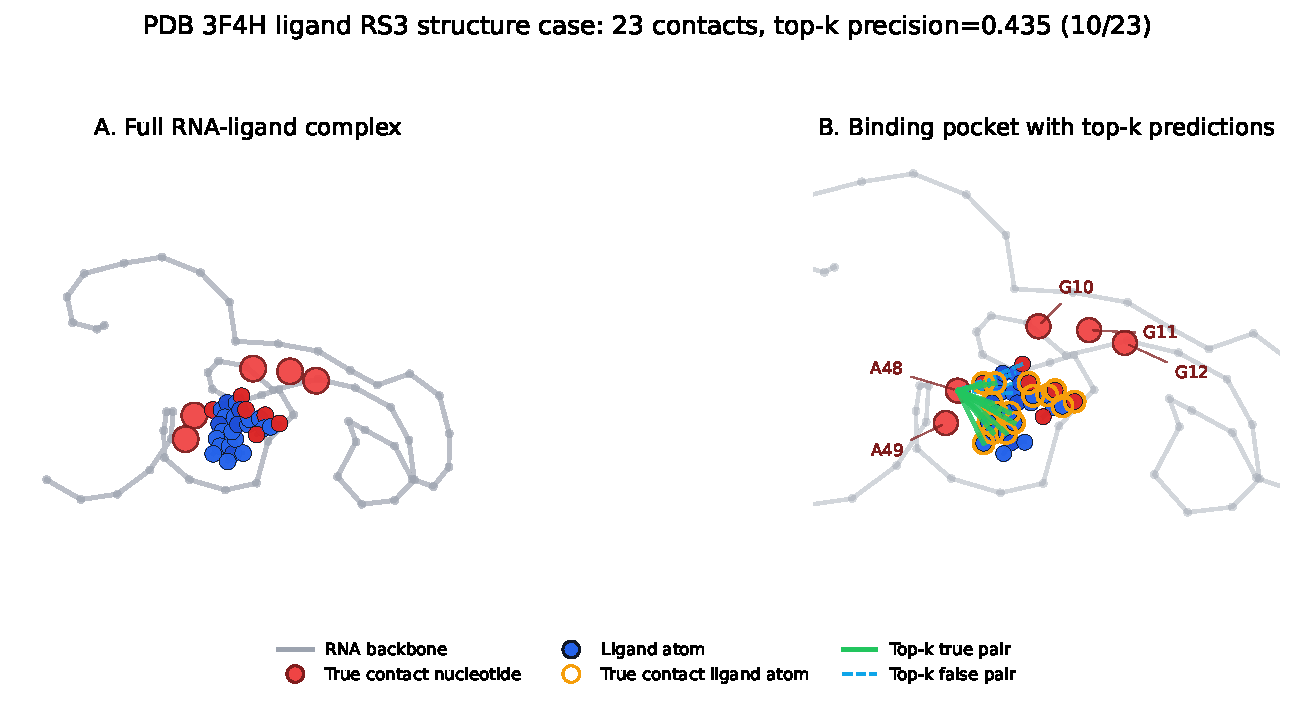
\includegraphics[width=0.95\linewidth]{fig_structure_case_3f4h.pdf}
\caption{3D structural case study for PDB 3F4H. Contact-positive RNA nucleotides and ligand atoms are highlighted to connect the matrix-level contact prediction with physical RNA-ligand geometry.}
\label{fig:structure_case}
\end{figure}

Mapping the same predicted region onto the 3D RNA-ligand structure provides a more direct biological interpretation. The highlighted RNA nucleotides form a local binding region around the ligand, and several high-probability ligand atoms correspond to atoms positioned near the RNA surface. This case study should not be interpreted as exact binding-site localization. Rather, it suggests that contact supervision can enrich probability mass in physically plausible RNA-ligand regions and partially recover true contact features, which may help bridge global affinity prediction and structure-guided interpretation.

\subsection{Comparison with Existing RSMA Models}

DeepRSMA reported strong five-fold cross-validation performance on R-SIM, outperforming conventional machine learning methods such as support vector machines, random forests, XGBoost, and deep baselines adapted from protein-ligand affinity prediction.\cite{Hearst1998SVM,Breiman2001RandomForests,Chen2016XGBoost,Abbasi2020DeepCDA,Wang2021DeepDTAF,Nguyen2021GraphDTA,Huang2024DeepRSMA} DeepMIF further improved the published benchmark by enhancing multiview interaction modeling and maintaining separate information channels before fusion.\cite{Song2026DeepMIF}

StructRSMA is positioned differently. It is not intended to replace DeepRSMA or DeepMIF under the official five-fold benchmark protocol in the present study. Instead, it tests an orthogonal hypothesis: whether external RNA-ligand structural information can serve as an auxiliary supervision signal for pair-level affinity models. This makes the contribution complementary to multiview architectural improvements. In principle, contact pretraining and SCA could be combined with stronger future backbones, including DeepMIF-like multiview interaction modules, because the contact task operates at the nucleotide-atom level and does not depend on a specific global affinity head.

\subsection{Limitations}

Several limitations should be noted. First, the current study uses a local independent-test reproduction protocol and retrospective checkpoint-selection views rather than the official five-fold cross-validation or blind-test protocols used by prior RSMA benchmarks. The results should therefore be interpreted as proof-of-concept evidence and not as a direct SOTA comparison. Second, the PDB-derived contact set is modest in size and likely biased toward well-studied RNA motifs, crystallizable complexes, and ligands represented in structural databases. The de-overlap experiment confirms that strict removal of samples similar to the independent-test distribution substantially weakens downstream affinity transfer, indicating that coverage and distributional proximity of the structural pretraining set matter. Third, the 4 \AA{} contact threshold is simple and interpretable but does not distinguish hydrogen bonding, stacking, electrostatic contacts, hydrophobic contacts, or water-mediated interactions. Fourth, SCA compresses the predicted contact map into four summary statistics, which reduces overfitting risk but discards much of the pairwise geometric information. Fifth, although a random-SCA capacity control was included, finer-grained SCA ablations, such as removing individual contact statistics, testing frozen versus trainable contact heads, or comparing alternative contact-map pooling strategies, remain necessary for a fuller mechanistic understanding.

\section{Conclusions}

We introduced StructRSMA as a proof-of-concept framework for PDB-derived contact-supervised transfer in RNA-small molecule binding affinity prediction. The method preserves the original DeepRSMA four-view backbone and cross-fusion module, adds nucleotide-atom contact pretraining from RNA-ligand structures, and uses SCA to convert inferred contact priors into residual affinity calibration. True-contact and shuffled-contact controls show that PDB-derived contact maps contain learnable structural signal. Downstream affinity experiments under the local reproduction protocol indicate that contact pretraining can improve the transferred DeepRSMA representation, whereas SCA mainly reduces absolute prediction error. De-overlap and random-SCA controls further show that the observed behavior depends on structural contact supervision, distributional coverage of the PDB contact set, and residual calibration, rather than on an uncontrolled increase in model capacity alone. Qualitative contact-map and 3D structure visualizations suggest enrichment of probability mass in physically plausible RNA-ligand regions. Together, these results support the value of exploring available RNA-ligand structures as contact-level supervision for affinity datasets that contain only pair-level labels, while also emphasizing that the downstream benefit is distribution-sensitive.

\bibliography{structrsma_jcim}

\end{document}

